\documentclass{beamer}
\usetheme{ConnectivityLab}
\usepackage{times}
\usepackage{graphicx}
\usepackage{verbatim}
\usepackage{outlines}
\usepackage{fancyhdr}
\usepackage{subfigure}
\usepackage{cancel}
\usepackage{bibentry}
\usepackage{varwidth}
\usepackage{etoolbox}
\usepackage{epstopdf}
%%%%%%%%%%%%%%%%%%%%%%%%%%%%%%%%%%%%%%%%%%%%%%%%%%%%%%
%%%%%%%%%%%%%%%%%%%%%%%%%%%%%%%%%%%%%%%%%%%%%%%%%%%%%%

\title {
    Progress report
}
\author {
    Yin-Hong, Hsu
}
\date {
    05 24, 2017
}

%%%%%%%%%%%%%%%%%%%%%%%%%%%%%%%%%%%%%%%%%%%%%%%%%%%%%%
%%%%%%%%%%%%%%%%%%%%%%%%%%%%%%%%%%%%%%%%%%%%%%%%%%%%%%

\begin{document}
\begin{frame}
    \titlepage
\end{frame}

%%%%%%%%%%%%%%%%%%%%%%%%%%%%%%%%%%%%%%%%%%%%%%%%%%%%%%
%%%%%%%%%%%%%%%%%%%%%%%%%%%%%%%%%%%%%%%%%%%%%%%%%%%%%%

\begin{frame}{Outline}
    \tableofcontentsgather
    \tableofcontents
\end{frame}

%%%%%%%%%%%%%%%%%%%%%%%%%%%%%%%%%%%%%%%%%%%%%%%%%%%%%%
%%%%%%%%%%%%%%%%%%%%%%%%%%%%%%%%%%%%%%%%%%%%%%%%%%%%%%
\section{Wearable plan}

\begin{frame}{Function modification}
    \begin{itemize}
        \item {New UI flow}
        \item {Bracelet}
        \begin{itemize}    
            \item[-]{Seek Bracelet - change the notification way to the alarm instead of vibrate}
            \item[-]{Color Detection - new data format}
            \item[-]{Distance Detection - the bracelet only work well once}
            \item[-]{Power Information - hard code in bracelet}
            \item[-]{Connection switch - new connect and disconnect approach in new design}
        \end{itemize}
        \item {New layout, and new layout...}
    \end{itemize}
\end{frame}
\begin{frame} {New layout}  
    \begin{figure}[t]
    \centering
    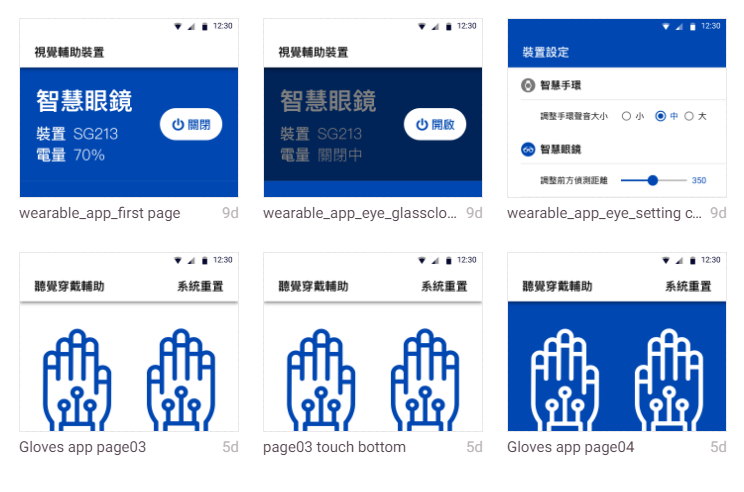
\includegraphics[width=0.8\textwidth]{figures/layout.png}
    \setbeamerfont{caption}{size=\tiny}
    \caption{They change the UI for several times}
    \end{figure}
\end{frame}
\begin{frame} {New UI flow}  
    \begin{figure}[t]
    \centering
    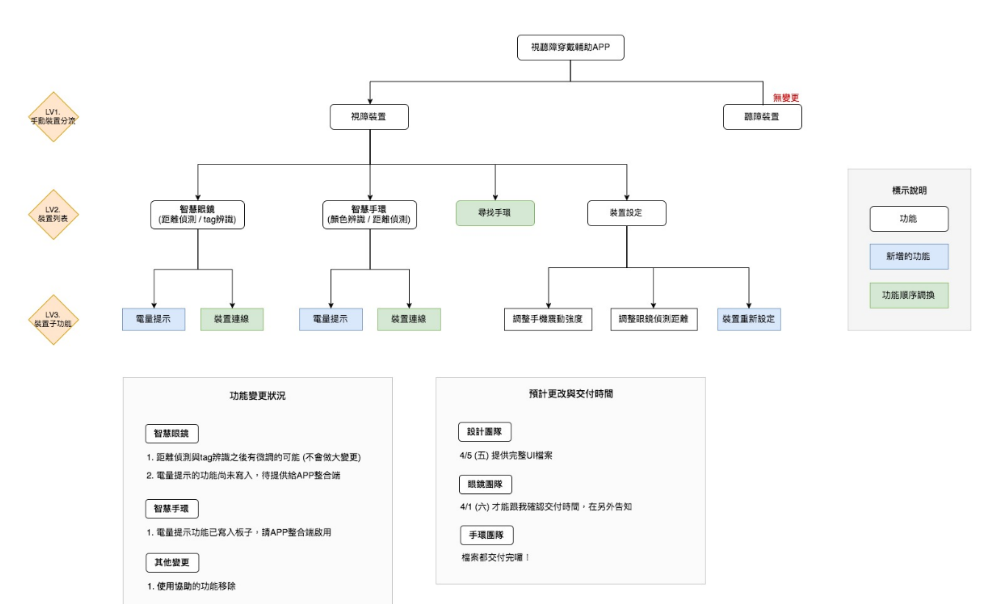
\includegraphics[width=0.8\textwidth]{figures/uiflow.png}
    \setbeamerfont{caption}{size=\tiny}
    \end{figure}
\end{frame}
\begin{frame} {Color detection - format}  
    \begin{figure}[t]
    \centering
    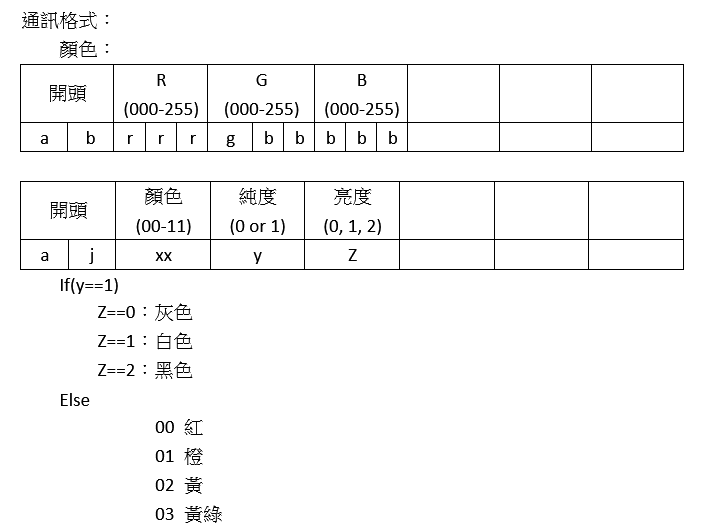
\includegraphics[width=0.8\textwidth]{figures/commformat.png}
    \setbeamerfont{caption}{size=\tiny}
    \end{figure}
\end{frame}


\end{document}
